\section{Introduction}
\label{sec:intro}

Digital watermarking is an important technique to 
protect the copyrights of digital products such as images, audios and
videos. A watermark is small amount of digital noise 
embedded into the digital representation of the products. 
%Like traditional watermarks (such as the one in Figure \ref{fig:banknote}),
%it often takes some special efforts (e.g., an algorithm) to plant
%a watermark into a product and to detect 
%whether a given product contains a watermark. The watermarking
%process typically consists of two steps: insertion of the watermarks into
%the original product and detection of the watermarks in a suspicious
%copy of the product or its variants.
%
%\begin{figure}[th]
%\centering
%\epsfig{file=notemark.eps, width=0.85\columnwidth}
%\caption{Watermark in a \$100 US Bank Note}
%\label{fig:banknote}
%\end{figure}
%
Watermarking is different from encryption, another method used to 
protect digital content from unauthorized access. Watermarks embedded 
in a product should not be {\em perceived} by the user or the application and hence 
don't affect the normal use of the product, whereas encrypted product cannot
be used unless the user has the means to decrypt the product, usually
with the help of a secret key.
Once the content is decrypted, unlimited illegal copies of the 
product can be made and used as if they were legal copies. Digital 
watermarking complements encryption. By embedding 
some watermarks that are hard to remove, one can always claim the ownership 
of the product after detecting the watermarks. 
%Digital watermarking process has the following common properties. 
%
%\begin{enumerate}
%\item 
%The watermark information is a noise added to the original
%data, and the utility of the data must not be affected by the noise. 
%%quality of the original data. But this degration should not be 
%%perceived by the applications. The key point to keep the quality of 
%%the altered dataset is to 
%%constrain the negative effect of redundant information on
%% the original data. Different applications require different 
%%methods of evaluating the data quality. 
%Application-dependent utility metrics are 
%needed in association with different digital 
%watermark approaches. 
%\item 
%should be encoded into the
%original data with some random approach that depends on
%some secret keys and the watermarking data itself in order
%for the watermark to be resistant to malicious or benign attacks.
%\item 
%Third, in order to distinguish data with a watermark from data without 
%a watermark, a watermarking process must guarantee a low false positive 
%rate. That means that it should keep low rate of detecting unwatermarked 
%data as watermarked data. 
%\end{enumerate}

\begin{figure}[th]
\centering
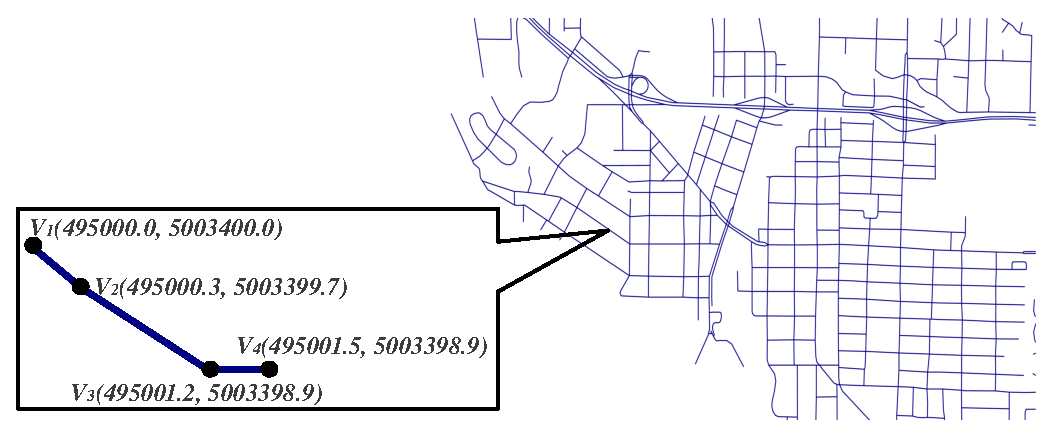
\epsfig{file=images/map.eps,width=0.9\columnwidth}
\caption{A Digital Road Map for Part of Anoka County, MN}
\label{fig:anoka}
\end{figure}

In this paper, we are concerned with the protection of copyrights of
digital road maps by watermarking. A digital road map is a vector graph
representation of roads in a geographical region. Such maps are 
widely used in Geographic Positioning Systems (GPS) and other GIS or
location-based applications.
Figure \ref{fig:anoka} shows an example of a snippet of a
road map of Anoka County, MN in the United States. 
In this map, a road is represented by a {\em polyline}, 
shown in the blow-up image, where a polyline is a sequence of connected
straight line segments. Each line segment is presented digitally by its
two end vertexes in terms of ($x$, $y$) coordinates, where $x$ and $y$ are
latitude and longitude of the point on earth, respectively. Very wide two-way
roads (e.g., freeways) with central dividers are represented by two (often)
parallel polylines, which are also shown in \figref{fig:anoka}.

\begin{figure}[th]
\centering
\epsfig{file=images/Flow.eps,width=0.6\columnwidth}
\caption{General Watermarking Framework For Road Maps}
\label{fig:workflow}
\end{figure}

The standard watermarking framework for digital road maps 
(shown in \figref{fig:workflow}) also adopts a two-step approach.
The two key modules in the framework are the watermark insertion
and detection algorithms. These two modules typically share some
common secret keys which are only known to the algorithms. Some
detection algorithms require the original map while others don't.
When digital road maps are unlawfully copied for commercial use,
they often undergo various modifications or transformations in hope that
the original watermarks are either removed or become undetectable.
Such modifications to the map is called {\em attacks} on the watermarks.
Existing attacks include attempts to remove or alter the watermarks, 
adding more noises to the map, cutting a map into smaller pieces or 
merging multiple maps from different sources. The last two attacks, which
we call ``{\em crop attack}'' and ``{\em merge attack}'' are less common, 
and they are the focus of our research in this paper.  

A scenario of a crop attack goes like this: an attacker obtains a big map, 
e.g., the map of the state of Minnesota, 
and crops out the Minneapolis - St.Paul area 
to create a ``new'' twin-city map. In the case of a merge attack, the attacker
extracts maps for various counties in Minnesota from several different
digital maps and composes a new Minnesota map by aligning these sub-maps
properly together. The first attack is easier to implement, while the second
attack is more difficult to carry out in practice and harder to defeat.
 
%For GIS spatial data,digital map, watermarking methods mean trying to find out the additional
%information,in other words 'watermark', which may be inserted into the very map
%before. So the watermarking process could be divided into two steps. First, owner
%of the map insert some watermark into the map with some secret strategies. Second,
%anytime when the owner gets a suspicious map, he can try to find the watermark with
%the same strategy as insertion. So the whole workflow of digital map watermarking can 
%be illustrated like Figure \ref{fig:workflow}.

%The spatial attributes of GIS spatial data such as digital
%road maps consist of numeric data that describe the positions 
%of spatial objects. The ShapeFile is a popular format to 
%store GIS spatial data. Figure \ref{fig:3} shows the spatial attributes
%of of digital road map of part of Anoka county.

Existing watermarking techniques come in two categories, 
{\em global watermarking} and {\em local watermarking}. 
In global watermarking,
%\cite{KhannaZ00, SionAP02, SionAP03, Kitamura01:DFT, Liyuanyuan03},
%which is a more common approach,
the insertion module computes an overall watermark based on 
the global information of the data, 
and inserts this watermark over the whole data. Detection requires
the reconstruction of the original watermark which requires
global information as well. As such, these techniques cannot handle
crop or merge attacks. 

%As a result,
%given a fragment of a map  (a crop) which contains just part of 
%the watermark, the detection module cannot conclusively determine 
%its ownership because 1) it doesn't
%have the complete information needed to compute the watermark, and 2)
%even if it can compute the complete watermark, matching it against part of
%the map can be problematic. For similar reasons,
%the global technique also doesn't handle merge attacks.
%%\KZ{Give a concrete example of a particular global watermarking technique
%%failing the crop attack, using either figure or formula to aid 
%%the explanation.}
%%A frequency domain watermarking approach\cite{Liyuanyuan03} insert 
%%watermark into coefficients of L-level DWT of the whole map. However,
%%if the watermarked map is cropped or merged with other map. The 
%%coefficients of DWT will be changed. Thus, this method will also 
%%be defeated by crop attack.

In local watermarking, % \cite{OhbuchiUE02,OhbuchiUE03,Voigt:2003}, 
the insertion module generates many watermarks
for different regions of the data, and each watermark is computed from the
local information of the corresponding regions. For example,  
one can partition a map into many smaller regions,
and insert a watermark according to the properties of 
the data in each region.
%The watermarking 
%information depends on a global structure and is dispersed globally. 
%A massive chop will beat this watermarking approach. 
%If the watermark 
%depends on local information and is dispersed locally, the watermarking 
%is classified as local. 
Local road map watermarking schemes \cite{OhbuchiUE02,OhbuchiUE03,Voigt:2003} have 
the potential of surviving crop attacks. However, to handle
``massive cropping'', i.e., cropping out a very small piece of the original map,
existing local schemes have to resort to fine-grained partitioning and
the insertion of many more watermarks which may affect the perception of the 
map. Moreover, many of these techniques
require coordination between the detection of watermarks in
adjacent sub-regions (e.g., some repetitive patterns) to conclude the 
authenticity of the overall map. Such coordination may fail if it happens
at the boundary of the cropping.
Such massive cropping attacks are real, since
in our previous example, the Twin-Cities area is much smaller than the whole
state of Minnesota. 
%none of them are robust enough (as we will discuss later in Section
%\ref{sec:related}) to handle ``massive cropping'' which means
%cropping . When this kind of attack
%happens, too many watermarked data will be removed.
%\KZ{Give example to show why a typical local watermarking scheme can't
%survive massive cropping and why are massive cropping and merge
%attacks very challenging?}

None of the existing local methods can defeat the merge attack because
all of them compute a global confidence score based on the watermarks
extracted from individual sub-regions. If a significant part of the map
comes from a foreign source without the inserted watermarks, these
methods typically give a low confidence score and fail to identify
part of the map as being authentic. Without a proper data structure,
these methods also suffer from high computation complexity if they attempt 
to ``guess'' where the watermarked region is in the map.

%?gwithout knowing the size or the location of the authetic fragment
%?gof the map, these methods easily confuses sub-regions without watermarks
%?gsince they can't effectively detect the watermark in
%?gpart of a given map. Hence, these merged data will act as enormous ``negative 
%?gnoise'' which defeats watermarking more easily.
%
%For example\cite{Voigt:2003}, when the watermarked map is ``massive'' cropped, 
%many ``patches'' that is marked may probably be
%removed. Thus $F$ distribution of watermarked points may be destroyed.
%And when the watermarked map is attacked by ``merge attack''. Many data points
%from other sources will be mistaken for possible watermarked points. Thus, 
%watermarking technique will more possibly fail.

%Few studies have considered the special properties of spatial attributes 
%in GIS spatial data, although there has been some researches on how to 
%insert watermarks into numeric data. For example, they all consider dispersing 
%the watermark globally. However, in GIS digital data, an easy method
%of attack is to cut a small piece of GIS spatial data and use
%only this piece.In a GIS digital data set, 
%a small part of a data set for a small region might still be valuable 
%and useful.  An attacker may want to use a small region
%of digital road maps for some applications, which is a "massive chop"
% attack. Thus, global watermarking is not a good approach to survive 
%this type of attack. Meanwhile, an attacker can also combine different 
%small parts from different maps and make a completely 'new' map. For example, 
%an attacker might only want the digital road 
%map for Minneapolis-St. Paul area from the Minnesota state map.
%Another attacker might want to extract maps for different
%counties in Minnesota from different digital road maps and
%compose a new digital road map covering all of Minnesota.This
%kind of attack, to our best knowledge, can defeat all the existing
%watermarking methods.

%To survive the "massive chop" attack and to some extent defeat the 'combination'
%attack, ur preferred watermarking technique for a GIS digital data set such as 
%a digital road map is local watermarking. 

In this paper, we propose a novel local watermarking approach which
partitions the original map by a modified quad-tree structure. The depth of
the tree is determined by the road density in the region.
We compute the local watermark for each partition by 
the total length of the roads in that partition and 
each watermark is represented by {\em one bit} change in the original data. 
During detection phase, our approach can reconstruct the quad-tree
and identify the potential locations of the embedded watermarks, and can
report with high confidence if a given attacked map (be it traditional
attacks or crop/merge attacks) contains a sub-region which carries the
original watermarks as well as reporting that sub-region itself. 
In addition, the detection method in our approach
doesn't require the original map,
but only needs a ``secret grid boundary'' which serves as the key. The size
of this key is negligible compared to the original data. Watermark detection
scheme without the need for original data is also known as ``blind
watermarking.''
 
%using the local information which is collected by a modified Quadtree model 
%to insert watermarks into the position data in the GIS spatial data. 
%The most important feature of our approach is, on one hand, 
%that the illegal usage of only a small part of GIS spatial data, 
%which defeats most current watermarking techniques, can be detected. 
%On other hand, since we construct the Quadtree according to 
%the density of road length, even for
%a merged map the structure of Quadtree will almost be the same.
%
%\subsection{Our Contributions}
This paper makes the following key contributions:
%\KZ{Jacky: expand these bullet a bit more where appropriate.}
\begin{itemize}
\item {\em The framework defeats massive cropping and merging
attacks with high accuracy.} Our experiments show that
our approach achieves 100\% detection accuracy for moderate
cropping and more than 80\% accuracy with more than 95\% of the original
map cropped, whereas the accuracy of two other state-of-the-art approaches
degrades to around 20\% with similar massive cropping. Our method outperforms
the peers by similar margins under merge attacks. 

%Many watermarking approaches are based on
%global information and hence don't survive cropping or merge attacks
%which are more difficult than common noise attack. For merge attacks,
%not only can we detect the authenticity of the map, we can also
%accurate pinpoint which part of a given map carries the watermark
%and is hence copied.

\item {\em The framework incurs little distortion.} 
%\KZ{need to say why we can accomplish this briefly.}
The map is partitioned into sub-regions of various sizes {\em on demand}. 
Watermarking position is calculated by information inside these sub-regions. 
We use a one-bit watermark to represent that the 
sub-region is watermarked.  Consequently, to effectively watermark the whole
Twin-Cities 7-counties map (23.5MB), our approach merely modified 
423 {\em bits}. 

\item {\em The framework is lightweight.} It is a blind watermarking method
which requires no original map for watermark detection, 
and the time complexity of both the insertion
and detection algorithm is $O(|V|log\LEN)$ where $|V|$ is the number of vertices in
the map and $\LEN$ is the total length of roads in the map.
\end{itemize}

The remainder of this paper is organized as follows. Section 
\ref{sec:problem}
 introduces some preliminaries about the watermarking GIS digital data
and formalizes the problems of interest. 
Section \ref{sec:appr}  
discusses the proposed digital watermarking approach in detail. 
Section \ref{sec:exper} describes the experiment setup and presents
evaluation results on a real digital map data set. 
Section \ref{sec:related} discusses the related work, and
we conclude the paper with some further work in section \ref{sec:conclude}.

%This paper focuses on the development of a novel GIS
%digital data watermarking approach. We consider the properties 
%of GIS digital data and the special kinds of attacks to
%which GIS digital data are vulnerable. Also, a case study on
%a digital road map is conducted to illustrate the performance
%of the proposed GIS digital data watermarking approach.
%
%%% Local Variables:
%%% mode: latex
%%% TeX-master: "paper"
%%% End:
